
\documentclass[11pt,A4]{article}
\usepackage[left=2 cm,right=2cm,top=2.5cm,bottom=2.5cm]{geometry}
\usepackage{blindtext}
\usepackage{amsmath}
\usepackage{amsfonts}
\usepackage{amssymb}
\usepackage{niceframe}
\usepackage{enumitem}
\usepackage{swrule}
\usepackage{ulem}
\usepackage{hyperref}
\usepackage{multicol}
\hypersetup{
    bookmarks=true,         % show bookmarks bar?     % links in new PDF window
    colorlinks=true,       % false: boxed links; true: colored links
    linkcolor=red,          % color of internal links (change box color with linkbordercolor)
    citecolor=green,        % color of links to bibliography
    filecolor=magenta,      % color of file links
    urlcolor=cyan           % color of external links
}
\usepackage{xcolor}
\usepackage{pgf,tikz}
\usepackage{mathrsfs}
\usetikzlibrary{arrows}
\usepackage{polyglossia}
\usepackage{varwidth,umrand}
\usepackage{nicefrac}
\usepackage{tcolorbox}
\tcbuselibrary{skins,listings,breakable}
\usepackage{listings}
\definecolor{ocre}{RGB}{65,105,225}
\definecolor{BrickRed}{RGB}{132,31,39}
\definecolor{RoyalBlue}{RGB}{243,102,25}
\usepackage{newverbs}
\newverbcommand{\cverb}{\color{blue}}{}
\lstset{language=[LaTeX]TeX,
,escapeinside=``,
	keywordstyle=\color{blue},%
	upquote=true,
columns=flexible,
texcsstyle=*\color{blue},
	 basicstyle=\small,
	stringstyle=\color{blue},
	commentstyle=\color{red}}	   
\lstset{moretexcs={question,part,pointsinrightmargin,mathbb,dfrac,subpart,subsection,subsubsection,abstractname,textsubscript,mathcal}}
%===================================================================
\tcbset{bicolor,colback=green!3!white,colbacklower=white,colframe=BrickRed}
%============================================================================
%===============================================================
\setdefaultlanguage[calendar=gregorian,,locale=algeria]{arabic}
\newfontfamily\arabicfont[Script=Arabic,Scale=1]{Amiri}
\newfontfamily\arabicfontsf[Script=Arabic,Scale=1.2]{Aljazeera}
\newfontfamily\arabicfonttt[Script=Arabic,Scale=1]{Times New Roman}
\setotherlanguage{english}
% ----------------------------------------------------------------





%--------------------------------------
\def\c{\char'} 
\font\G = umrandb at 20pt

\title{استعمال حزمة 
 exam
في 
كتابة مواضيع الامتحانات والفروض
بالعربية
}
\author{
\href{https://www.facebook.com/groups/573789572802504/?ref=bookmarks}{\LR{\LaTeX 4 ALL}}
}

\begin{document}
\artdecoframe{
\maketitle
}
\niceframe{
\tableofcontents}
\section{التعريف بحزمة { exam} }
 حزمة تستعمل في كتابة مواضيع الامتحانات والفروض في برنامج 
\LaTeX 
.\\
وهنا قمت باظافة بعض التنسيقات
على شكل حزمتين
\href{https://drive.google.com/open?id=1lOoPPxZE4uCbjJtLTnVITsyLAhPeWImx}{\LR{sexam \& wexam}}
 التي ستمكننا من استغلال امكانيات exam في الكتابة العربية ،
 يمكن تحميلهما من 
\href{https://drive.google.com/open?id=1lOoPPxZE4uCbjJtLTnVITsyLAhPeWImx}{\textbf{هنـــا}} 
.

  نتمنى أن يكون مفيدا للأخوة مستعملي 
\LaTeX
.
\section{ استعمال الحزمة sexam}
يجب أولا تحميل الحزمة
%بالنقر
%\href{http://mirrors.ctan.org/macros/generic/umrand.zip}{هنا} 
sexam
ووضعها مع ملف التاك الذي نكتب فيه موضوع الإمتحان.\\
ندرج في الديباجة الأمر :
\begin{english}
\begin{lstlisting}
\documentclass[12pt]{exam}
\usepackage{sexam}
\end{lstlisting}
\end{english}
%\newpage
\section{كتابة موضوع الامتحان }
\begin{enumerate}
\item
لتغيير نوع الخط الرئيسي أو الخطوط الثانوية ،نفتح ملف 
\LR{sexam.sty}
ثم نقوم بتغيير اسم الخطوط الموضحة في الصورة :
$$\fbox{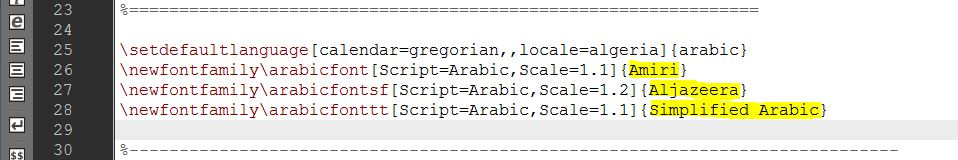
\includegraphics[width=16cm]{01.JPG}}$$
\item
بعد فتح ملف التاك الذي سنكتب فيه الامتحان نجد الأوامر التالية:
\begin{english}
\begin{lstlisting}
\newcommand{\lycee}{\sffamily `\textarabic{نكتب هنا اسم الثانوية}` }
\newcommand{\annee}{2018-2017}
\newcommand{\examnum}{ `\textarabic{نكتب اسم الامتحان أو الفرض مع السداسي الخاص به}`}
\newcommand{\examdate}{\date}
\newcommand{ \duree }{ `\textarabic{الحجم الساعي للامتحان}` }
\newcommand{ \niveau }{  `\textarabic{المستوى الذي سيمتحن}`}
\end{lstlisting}
\end{english}
نقوم بكتابة المعلومات الخاصة بنا ، كما في المثال التالي:
\begin{english}
\begin{lstlisting}
\newcommand{\lycee}{\sffamily `\textarabic{ثانوية الدكتور أحمد عروة}` }
\newcommand{\annee}{2018-2017}
\newcommand{\examnum}{ `\textarabic{امتحان الفصل الثاني مادة الرياضيات}`}
\newcommand{\examdate}{\date}
\newcommand{ \duree }{ `\textarabic{ساعتان}` }
\newcommand{ \niveau }{  `\textarabic{سنة ثانية تقني رياضي}`}
\end{lstlisting}
\end{english}
\item
بعد الديباجة نجد الأوامر التالية على شكل اختصارات قمنا بتعريفها سابقا ، نتركها كما هي :
\begin{english}
\begin{lstlisting}
{ \lycee}
%-----------------
\hfill
%-----------------
{\sffamily `\textarabic{ السنة الدراسية :}`\annee}
%-----------------
%-----------------
$\rule{\textwidth}{1pt}$

\vspace{9pt}
\centerline{\sffamily\large  \examnum}
%-----------------
$\rule{\textwidth}{1pt}$\\
{\sffamily `\textarabic{ الشعبة :}` \niveau  
 %-----------------
\hfill
%-----------------
`\textarabic{  المدة:}`\duree}
\end{lstlisting}
\end{english}
\item
بعد المعالجة نجد :
$$\fbox{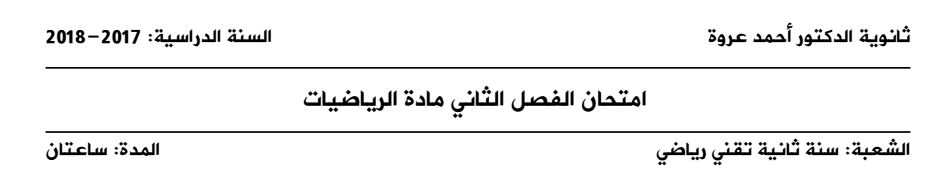
\includegraphics[scale=0.7]{2.JPG}}$$
\item
بعد ضبط العناوين الرئيسية للامتحان ، ننتقل إلى المضمون ألا وهو التمارين .\\
\begin{enumerate}[label=\alph*)]
\item
للبدء في كتابة التمارين نكتب الأمر :
\begin{english}
\begin{lstlisting}
\begin{questions}
....
\end{questions}
\end{lstlisting}
\end{english}
\item
لإدراج التمرين الأول نكتب الأمر :
\verb#\question[note]#
فيظهر لنا العنوان مرفقا بالتنقيط 
\LR{(note)}
الخاص به  :
 \begin{tcolorbox}[attach boxed title to top right=
{yshift=-\tcboxedtitleheight/3,xshift=-5mm},title=\textarabic{\sffamily مثال},colbacktitle=BrickRed,sidebyside]

\begin{flushright}
\uline{\textbf{\sffamily التمرين الأول :}}   
(1 نقطة)
\end{flushright}

\tcblower
نكتب الأمر
\begin{english}
\begin{lstlisting}
\begin{questions}
\question[1]
\end{questions}
\end{lstlisting}
\end{english}
\end{tcolorbox}
نفس الأمر إذا أردنا ادراج تمرين آخر.
 \begin{tcolorbox}[attach boxed title to top right=
{yshift=-\tcboxedtitleheight/3,xshift=-5mm},title=\textarabic{\sffamily مثال},colbacktitle=BrickRed,sidebyside]

\begin{flushright}
\uline{\textbf{\sffamily التمرين الأول :}}   
(1 نقطة)\\
\vspace{0.3cm}
\uline{\textbf{\sffamily التمرين الثاني :}}   
(3 نقاط)
\end{flushright}

\tcblower
نكتب الأمر
\begin{english}
\begin{lstlisting}
\begin{questions}
\question[1]
\question[3]
\end{questions}
\end{lstlisting}
\end{english}
\end{tcolorbox}
\item
للبدء في كتابة الأسئلة الرئيسية في التمرين نستعمل البيئة
parts
بعد الأمر :
\verb#\question[note]#
كما يلي :
\begin{english}
\begin{lstlisting}
\begin{questions}
\question[note]
\begin{parts}
%
\part[note] 
%
\end{parts}
\end{questions}
\end{lstlisting}
\end{english}
الأمر 
\verb#\part[note]#
معناه السؤال رقم 
1)
 في التمرين الأول مرفقا بتنقيطه note
.\\
إذا أردنا عدم ارفاق السؤال بتنقطيه نكتب :
\verb#\part#
فقط.

 \begin{tcolorbox}[attach boxed title to top right=
{yshift=-\tcboxedtitleheight/3,xshift=-5mm},title=\textarabic{\sffamily مثال},colbacktitle=BrickRed]
\begin{english}
\begin{lstlisting}
\begin{questions}
\question[3]
`\textarabic{لتكن الدالة }` $g$ `\textarabic{ المعرفة على}` $\mathbb{R}-\left\lbrace -1 \right\rbrace$ 
`\textarabic{بالعبارة : }` $g(x)=\dfrac{2x}{x+1}$
`\textarabic{وليكن }` $(C_g)$
`\textarabic{تمثيلها البياني في معلم متعامد ومتجانس }`
$\left( O;\vec{i}; \vec{j}\right)$.
%
\begin{parts}
\part[1]
`\textarabic{ بيّن أنه من أجل كل}` $x_0$ `\textarabic{من}` 
$\mathbb{R}-\left\lbrace -1 \right\rbrace$ :
$$\dfrac{g(x_0+h)-g(x_0)}{h}=\dfrac{2}{(x_0+h+1)(x_0+1)}$$
%
\part[1]
%
\part
\end{parts}
\end{questions}
\end{lstlisting}
\end{english}
\tcblower
\begin{center}
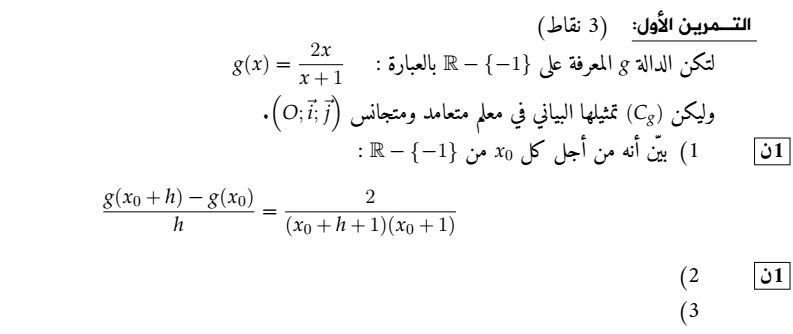
\includegraphics[width=14cm]{3.JPG} 
\end{center}

\end{tcolorbox} 
\item
يمكن ادراج الأسئلة الفرعية الخاصة بكل سؤال part في تمرين question 
وذلك بادراج البيئة
subparts
والأمر 
\verb#\subpart[note]#.
\begin{tcolorbox}[colback=white]
نكتب الأمر
\begin{english}
\begin{lstlisting}
\begin{questions}
\question[note]  % `\textarabic{التمرين الأول مرفق بنقطة}`
\begin{parts}    %
\part[note]      % `\textarabic{السؤال الأول في التمرين}`
\begin{subparts}
\subpart[note]   %   `\textarabic{السؤال الفرعي الأول الخاص بالسؤال رقم 1}` 
\end{subparts}
\end{parts}
\end{questions}
\end{lstlisting}
\end{english}
\end{tcolorbox}
\end{enumerate} 
%---
 \begin{tcolorbox}[attach boxed title to top right=
{yshift=-\tcboxedtitleheight/3,xshift=-5mm},title=\textarabic{\sffamily مثال},colbacktitle=BrickRed,sidebyside]
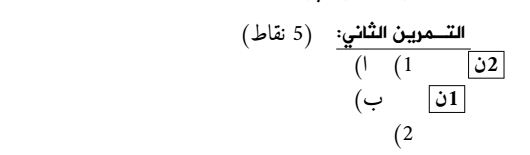
\includegraphics[width=6cm,height=5cm]{4.JPG} 
\tcblower

\begin{english}
\begin{lstlisting}
\question [5]

\begin{parts}
\part[2] 

\begin{subparts}
\subpart   % `\textarabic{السؤال الفرعي الأول الخاص بالسؤال رقم 1}` 
\subpart[1]
\end{subparts}

\part 

\end{parts}
\end{lstlisting}
\end{english}
\end{tcolorbox}
\item
يمكن تغيير موضع ظهور تنقيط الأسئلة إلى يسار الصفحة ،وذلك بإضافة الأمر
\verb#\pointsinrightmargin#
قبل بداية الأسئلة.
%--
 \begin{tcolorbox}[attach boxed title to top right=
{yshift=-\tcboxedtitleheight/3,xshift=-5mm},title=\textarabic{\sffamily مثال},colbacktitle=BrickRed,sidebyside]
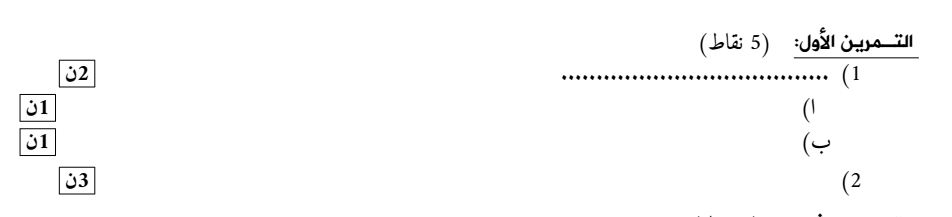
\includegraphics[width=7cm,height=5cm]{9.JPG} 
\tcblower

\begin{english}
\begin{lstlisting}
\pointsinrightmargin
\question [5]
\begin{parts}
\part[2]  ......................................

\begin{subparts}
\subpart[1] % `\textarabic{السؤال الفرعي الأول الخاص بالسؤال رقم 1}` 
\subpart[1]
\end{subparts}

\part[3]

\end{parts}
\end{lstlisting}
\end{english}
\end{tcolorbox}


\end{enumerate}
\subsection{ترقيم الصفحات}
يكون بشكل آلي اظهار رقم الصفحة مع عبارة تغييرها اذا كان الموضوع مكونا من صفحتين.
$$
\includegraphics[width=12cm]{6.JPG} $$
$$
\includegraphics[width=12cm]{7.JPG} $$
أما إذا كان مكونا من صفحة واحدة فقط يظهر:
$$
\includegraphics[width=12cm]{8.JPG} $$
\section{اختبار باستعمال sexam }
$$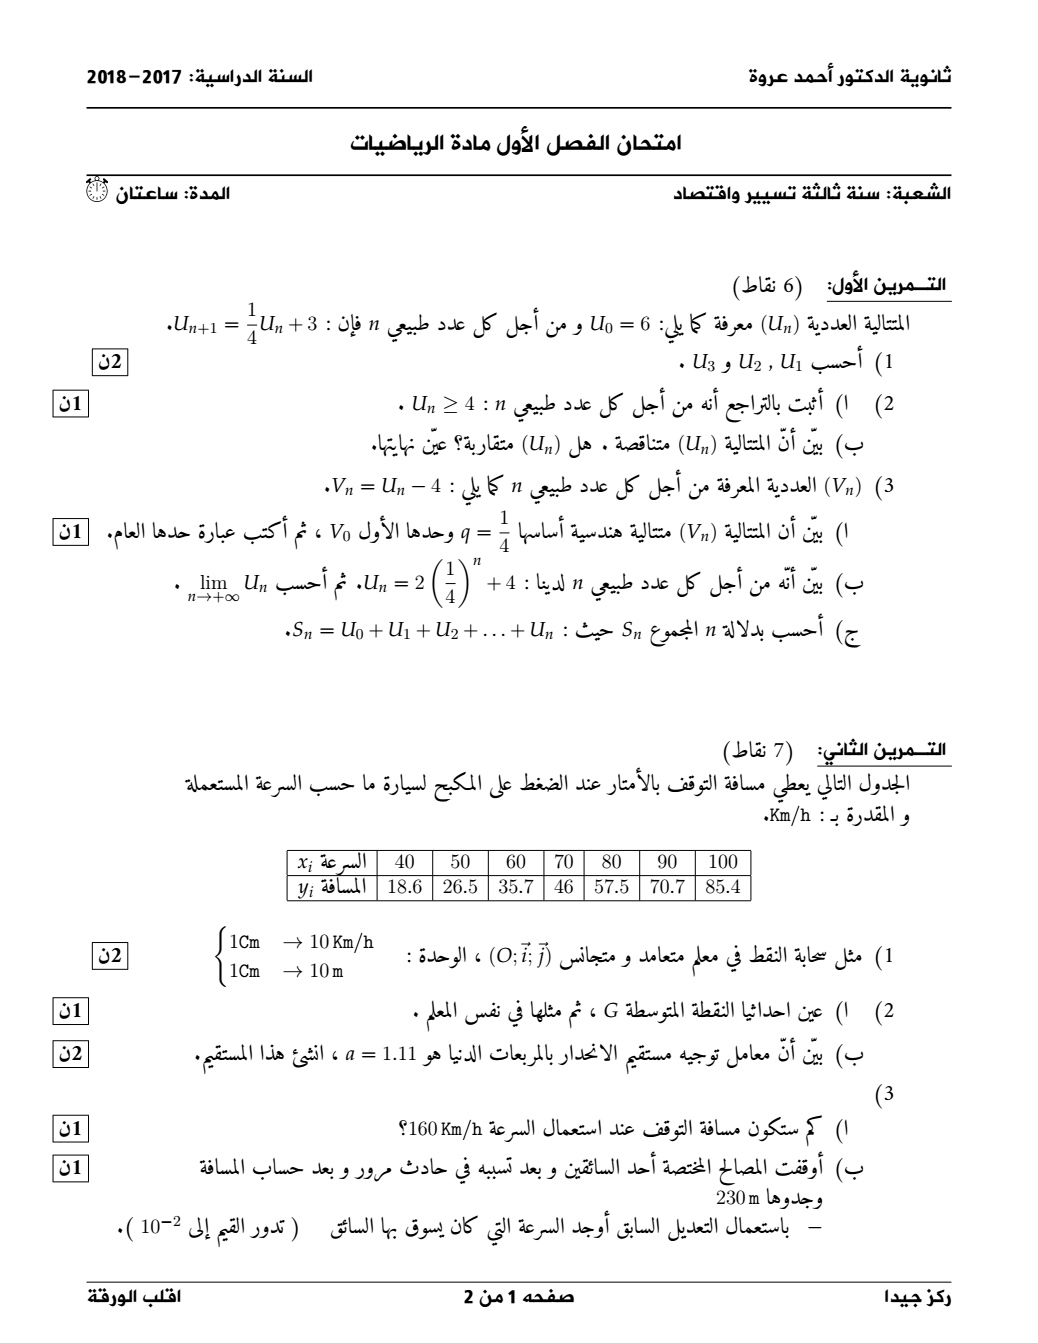
\includegraphics[width=14cm]{10.png}  $$

\section{اختبار باستعمال wexam }
لها نفس مبدء عمل sexam ، لكنها تظهر الأطار.
$$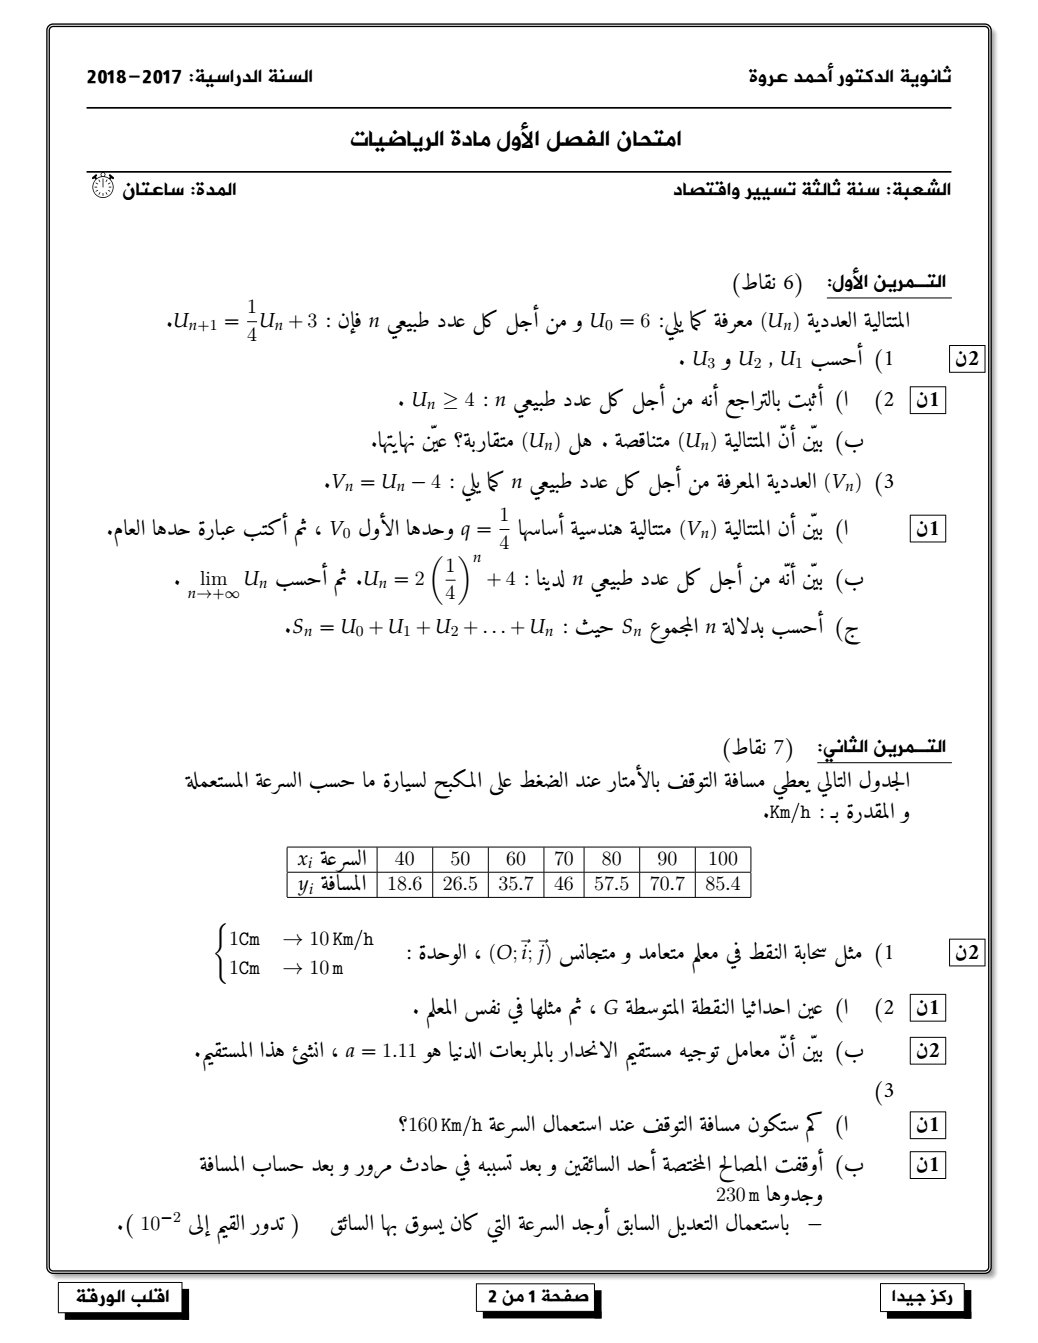
\includegraphics[width=14cm]{11.png}  $$
\end{document}